%==============================================================================
%  Effect of an authored joint-limit prior on multi-view pose regression
%  SMILify / SMILySTICKS -- internship report
%  Compile:  pdflatex mv_study.tex  (twice, for cross-references)
%==============================================================================
\documentclass[11pt,a4paper]{article}

\usepackage[T1]{fontenc}
\usepackage[utf8]{inputenc}
\usepackage{lmodern}
\usepackage[english]{babel}
\usepackage[margin=2.5cm]{geometry}
\usepackage{amsmath,amssymb}
\usepackage{graphicx}
\usepackage{booktabs}
\usepackage{multirow}
\usepackage{siunitx}
\usepackage{caption}
\usepackage{subcaption}
\usepackage{enumitem}
\usepackage{xcolor}
\usepackage[hidelinks]{hyperref}
\usepackage{cleveref}

\sisetup{
  detect-weight = true,
  detect-family = true
}

\captionsetup{font=small,labelfont=bf}
\captionsetup[sub]{font=small}
\graphicspath{{figures/}}

\emergencystretch=2em

\newcommand{\lam}{\lambda}
\newcommand{\best}[1]{\textbf{#1}}
\newcommand{\armref}{\textsc{mv-ref}}
\newcommand{\svref}{\textsc{sv-ref}}

\title{\textbf{Effect of an Authored Joint-Limit Prior on\\
Multi-View 3D Pose Regression of the Stick Insect}\\[0.4em]
\large A regularisation sweep on the SMILySTICKS benchmark, and a comparison
with the single-view case}

\author{%
  Youness ANOUAR\\
  \small Forschungszentrum J\"ulich --- SMILify project
}

\date{10 September 2026}

%==============================================================================
\begin{document}
\maketitle


\noindent\rule{\textwidth}{0.4pt}

%==============================================================================
\section{Introduction}
\label{sec:intro}

The single-view companion study \cite{sv} established that an authored
per-joint rotation prior removes almost all anatomically impossible poses from
the SMILify stick-insect regressor, and that the accuracy cost of doing so is
small but systematic. It also left one question open by construction: the
single-view problem is underdetermined, so a prior that restricts the solution
set is doing work the image evidence cannot do. If the ambiguity is the reason
the prior helps, then a model that already resolves depth from geometry should
have less to gain --- and, because its remaining freedom is genuinely
constrained by data rather than by chance, more to lose.

The multi-view regressor is exactly that test case. It observes the same animal
from up to five calibrated, synchronised cameras, and triangulation pins the 3D
configuration far more tightly than a single \(224\,\)px crop can. The study
reported here asks:

\begin{quote}
\emph{Does the authored joint-limit prior remain worthwhile once multi-view
geometry has already resolved most of the pose ambiguity?}
\end{quote}

The working hypothesis, stated in \cite{sv} and tested here, was that the
multi-view arm should show \emph{fewer violations to fix and a smaller benefit
from fixing them}. It does --- but the more consequential result is on the
other side of the ledger, and it is the reverse of the single-view finding.
This report gives:

\begin{enumerate}[nosep,leftmargin=1.6em]
  \item the plausibility/accuracy trade-off over four decades of $\lam$, in
        which --- unlike the single-view sweep --- the unregularised reference
        is the most accurate arm on \emph{every} metric
        (\Cref{sec:res-plaus,sec:res-acc});
  \item a range-of-motion analysis showing that the multi-view reference is
        already substantially more plausible than the single-view one, and that
        the same learned-margin over-regularisation nevertheless appears
        (\Cref{sec:res-rom});
  \item a controlled single-view/multi-view comparison, and the reading of the
        two sweeps that it supports (\Cref{sec:compare}).
\end{enumerate}

%==============================================================================
\section{Method}
\label{sec:method}

\subsection{Model and data}

All arms use the multi-view SMILify regressor: a
\texttt{vit\_large\_\allowbreak patch16\_224} backbone shared across views, per-view
learned view embeddings, a transformer-decoder head of hidden dimension
$1024$, a 6D rotation representation, and delta prediction from
ground-truth camera parameters. The model consumes up to $5$ views
(canonical camera order \texttt{A}--\texttt{E}) and emits one pose per
sample rather than one per view.

The benchmark dataset is identical to that of the single-view study:
\texttt{SMILySTICKS\_\allowbreak centred\_\allowbreak reprojected\_\allowbreak FIXED.h5}, \num{101250} samples over
$6$ sessions and $5$ synchronised cameras (\num{506250} view-items), with
undistorted images, reprojected 2D keypoints, 3D keypoints in SMAL joint order
and per-view camera intrinsics and extrinsics. The split is the same
camera-centric, sample-grouped split with seed $42$
($\num{86062}/\num{5062}/\num{10126}$ for train/validation/test); scoring
therefore covers \num{10126} multi-view samples, \num{424564} 3D joint errors
and \num{2121534} 2D joint errors. Images are processed at $224\,$px and 2D
errors are additionally reported at the native override resolution
$1530\times1530$.

Because the split, the dataset and the authored ranges are shared with
\cite{sv}, the single-view and multi-view numbers in \Cref{sec:compare} are
directly comparable: the only difference between the two studies is how many
views the network is allowed to see.

\subsection{Joint-limit regularisation}

The penalty is unchanged. Let $\theta_{a}$ denote the predicted Euler angle on
rotation axis $a$ and $[\,m_a, M_a\,]$ the authored range for that axis
(\texttt{3D\_model\_prep/\allowbreak SMILy\_\allowbreak STICK\_\allowbreak limits\_\allowbreak authored.pkl},
$55$ joints,
$162$ rotation axes). The term added to the training objective is the mean
one-sided hinge over all axes and all samples in the batch,
\begin{equation}
  \mathcal{L}_{\text{limit}}
  \;=\;
  \lam \cdot
  \frac{1}{|\mathcal{A}|}\sum_{a \in \mathcal{A}}
  \Big[
    \operatorname{relu}\!\big(\theta_a - M_a\big)
    \;+\;
    \operatorname{relu}\!\big(m_a - \theta_a\big)
  \Big],
  \label{eq:penalty}
\end{equation}
so that $\mathcal{L}_{\text{limit}} = 0$ whenever every axis lies inside its
authored box, and \Cref{eq:penalty} has \emph{zero gradient in the interior} of
the feasible set. The penalty is applied to the single pose the multi-view head
predicts, not per view; it therefore competes with the pooled evidence of all
five cameras at once, which is the mechanism proposed in
\Cref{sec:disc-mechanism}.

\subsection{Experimental arms}

\begin{table}[t]
\centering
\small
\caption{The five scored arms. Each constrained arm continues the reference
checkpoint for $24$ additional epochs with the penalty of \Cref{eq:penalty}
enabled. The reference received no additional epochs; \Cref{sec:disc-confound}
explains why, in the multi-view case, this asymmetry strengthens rather than
weakens the conclusion.}
\label{tab:arms}
\begin{tabular}{llccl}
\toprule
Arm & Mode & $\lam$ & Epoch & Checkpoint \\
\midrule
\armref{}            & multi-view & $0$       & 345 & \texttt{SMILySTICKS\_ViT\_model.pth} \\
\textsc{mv-1e-4}     & multi-view & $10^{-4}$ & 369 & \texttt{multiview\_lam1e-4/\dots\_0369.pth} \\
\textsc{mv-1e-3}     & multi-view & $10^{-3}$ & 369 & \texttt{multiview\_lam1e-3/\dots\_0369.pth} \\
\textsc{mv-1e-2}     & multi-view & $10^{-2}$ & 369 & \texttt{multiview\_lam1e-2/\dots\_0369.pth} \\
\textsc{mv-1e-1}     & multi-view & $10^{-1}$ & 369 & \texttt{multiview\_lam1e-1/\dots\_0369.pth} \\
\bottomrule
\end{tabular}
\end{table}

\Cref{tab:arms} lists the five scored arms. The four constrained arms share a
common starting point, epoch count and schedule and differ only in $\lam$, so
comparisons \emph{between} them are clean. The fine-tune budget here is $24$
epochs against the $49$ of the single-view study; this matters only for the
size of the confound discussed in \Cref{sec:disc-confound}, not for its
direction.

\subsection{Metrics}
\label{sec:metrics}

The metric definitions are those of \cite{sv} and are restated briefly so that
this report can be read on its own.

\paragraph{Anatomical plausibility.}
For each of the $162$ authored axes we report the fraction of test frames on
which the predicted angle falls outside $[\,m_a, M_a\,]$ (\emph{violation
rate}), and the signed distance beyond the nearer bound on violating frames
(\emph{overshoot}). Of the $162$ axes, $129$ carry a finite authored range; the
remaining $33$ are unconstrained by construction and contribute zero.
Aggregates quoted as ``over $162$ axes'' follow the convention of the sweep
tables; the ROM analyses of \Cref{sec:res-rom} are restricted to the $129$
bounded axes, whose mean authored range is \SI{51.6}{\degree}.

\paragraph{Accuracy.}
MPJPE and its percentiles in millimetres; PCK curves and mean/median 2D error
in pixels at both the native override resolution and the network input
resolution, since PCK@$N$\,px is resolution-dependent.

\paragraph{Range of motion and the clipping bound.}
For each bounded axis, ROM is the observed angular range
$\max_t \theta_a(t) - \min_t \theta_a(t)$ over the test set. To separate
``removing violations'' from ``shrinking motion'' we reuse the \emph{clipping
bound}: the ROM the reference arm would retain if its trajectory were merely
clipped into the authored box,
\begin{equation}
  \mathrm{ROM}^{\text{clip}}_a
  = \max\!\Big(
      \min\big(\max_t \theta_a(t),\, M_a\big)
      - \max\big(\min_t \theta_a(t),\, m_a\big),
      \; 0
    \Big).
  \label{eq:clip}
\end{equation}
An arm whose ROM sits \emph{above} $\mathrm{ROM}^{\text{clip}}$ has not fully
removed its violations; an arm whose ROM sits \emph{below} it has given up
motion inside the feasible set, where the penalty exerts no force.

%==============================================================================
\section{Results}
\label{sec:results}

\begin{table}[t]
\centering
\small
\setlength{\tabcolsep}{3.2pt}
\caption{Main results on the multi-view test split. Bold marks the best value
across all arms. Lower is better for violation, overshoot, MPJPE and 2D error;
higher is better for PCK. The reference row is set apart: it did not receive the
$24$ additional epochs. Unlike the single-view case, the reference achieves the
best 2D and 3D accuracy, while stronger joint-limit regularization substantially
improves anatomical plausibility.}
\label{tab:main}
\begin{tabular}{l c c *{9}{r}}
\toprule
 & & & \multicolumn{4}{c}{Anatomical plausibility}
 & \multicolumn{2}{c}{3D accuracy}
 & \multicolumn{3}{c}{2D accuracy} \\
\cmidrule(lr){4-7}\cmidrule(lr){8-9}\cmidrule(lr){10-12}
Arm & $\lam$ & Ep. &
\#viol. & rate & mean ov. & max ov. &
MPJPE & med. &
PCK@5 & PCK@5 & 2D err. \\
 & & &
axes & (\%) & (deg) & (deg) &
(mm) & (mm) &
nat. & 224 & (px) \\
\midrule
\armref{}        & 0         & 345 & 76 & 13.9595 & 2.647 & 56.57
                 & \best{0.9639} & \best{0.8382}
                 & \best{0.3350} & \best{0.9915} & \best{8.725} \\
\midrule
\textsc{mv-1e-4} & $10^{-4}$ & 369 & 75 & 4.6005 & 0.442 & 43.44
                 & 0.9920 & 0.8618 & 0.3260 & 0.9907 & 8.985 \\
\textsc{mv-1e-3} & $10^{-3}$ & 369 & 73 & 0.5365 & 0.012 & 17.65
                 & 1.0750 & 0.9475 & 0.2862 & 0.9882 & 9.724 \\
\textsc{mv-1e-2} & $10^{-2}$ & 369 & 57 & 0.0517 & 0.001 & 4.90
                 & 1.1414 & 1.0151 & 0.2511 & 0.9863 & 10.319 \\
\textsc{mv-1e-1} & $10^{-1}$ & 369 & \best{21} & \best{0.0073}
                 & \best{0.000} & \best{3.96}
                 & 1.2111 & 1.0624 & 0.2355 & 0.9820 & 10.942 \\
\bottomrule
\end{tabular}
\end{table}

\begin{figure}[t]
\centering
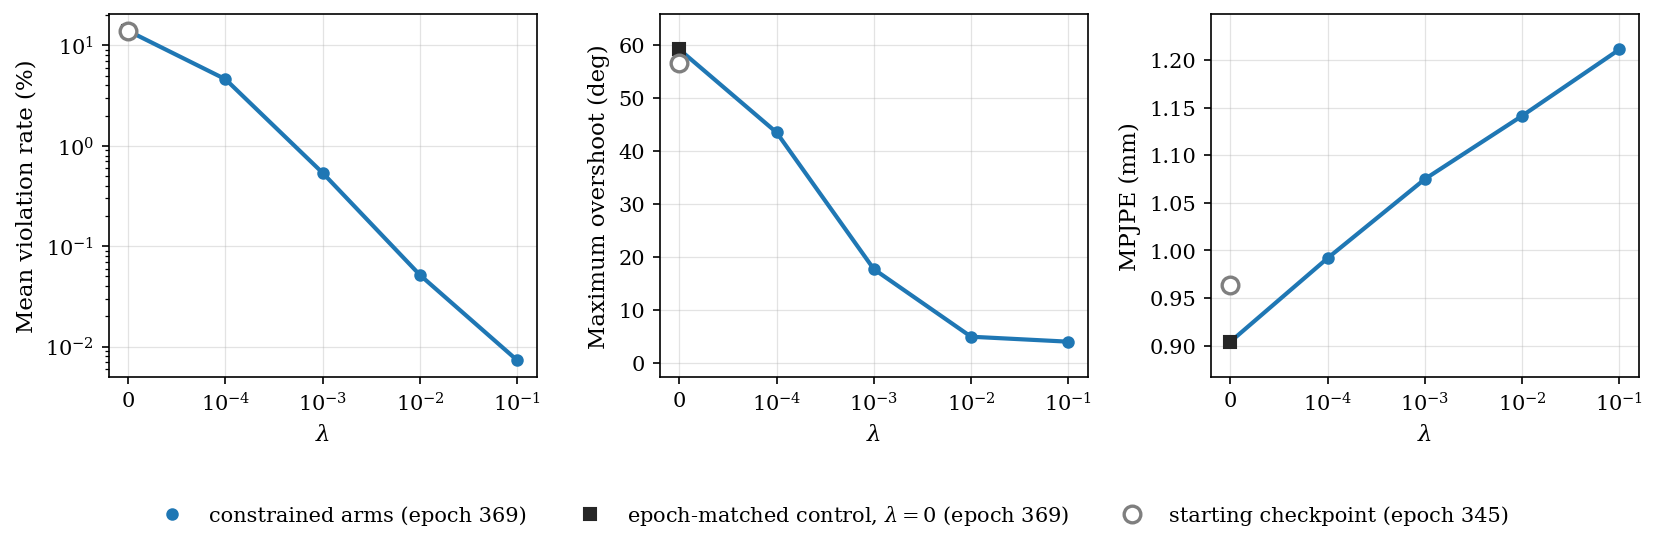
\includegraphics[width=\textwidth]{fig_mv_tradeoff.pdf}
\caption{The plausibility/accuracy trade-off across four decades of $\lam$.
Violation rate is the mean fraction of frames outside the authored range over
the $162$ authored axes (log scale). As in the single-view sweep neither curve
has an interior optimum; unlike the single-view sweep, the MPJPE curve rises
monotonically from the reference itself, so the accuracy cost of the prior is
directly visible rather than masked by continued training. The reference arm is
drawn as an open marker joined by a dashed segment because it did not receive
the $24$ additional epochs.}
\label{fig:tradeoff}
\end{figure}

\subsection{Anatomical plausibility}
\label{sec:res-plaus}

The prior is effective on the quantity it penalises (\Cref{tab:main},
\Cref{fig:tradeoff}). Relative to the reference, the mean violation rate falls
by a factor of $3.0$ at $\lam = 10^{-4}$, by $26$ at $10^{-3}$, by $270$ at
$10^{-2}$ and by $\approx\!1900$ at $10^{-1}$. Mean overshoot on violating axes
falls from \SI{2.65}{\degree} to below \SI{0.001}{\degree}.

As in the single-view study, the number of axes violating \emph{at least once}
is a poor summary: it falls only from $76$ to $21$ while the rate falls by more
than three orders of magnitude, because it is a binary indicator over
\num{10126} frames that a single marginal frame is enough to trip. The
informative quantity is again the maximum overshoot, which measures how badly
the worst predicted pose fails:
$56.6 \rightarrow 43.4 \rightarrow 17.6 \rightarrow 4.9 \rightarrow
\SI{4.0}{\degree}$. A requirement of the form ``no anatomically impossible pose
ever'' is met from $\lam = 10^{-2}$ upwards; at $\lam = 10^{-4}$ the model still
produces a \SI{43.4}{\degree} violation somewhere in the test set.

Two features distinguish the multi-view reduction curve from its single-view
counterpart. First, the reduction is \emph{slower} per decade at the low end:
$\lam = 10^{-4}$ divides the violation rate by $3.0$ in multi-view against
$5.4$ in single-view, and leaves $\SI{4.60}{\percent}$ of frames violating
against $\SI{2.73}{\percent}$. Second, it \emph{saturates} earlier at the high
end: the last decade buys only \SI{4.9}{\degree} $\rightarrow$
\SI{4.0}{\degree} of maximum overshoot, against $7.2 \rightarrow
\SI{2.5}{\degree}$ in single-view. The prior is fighting a stronger data term
in both regimes.

\begin{figure}[t]
\centering
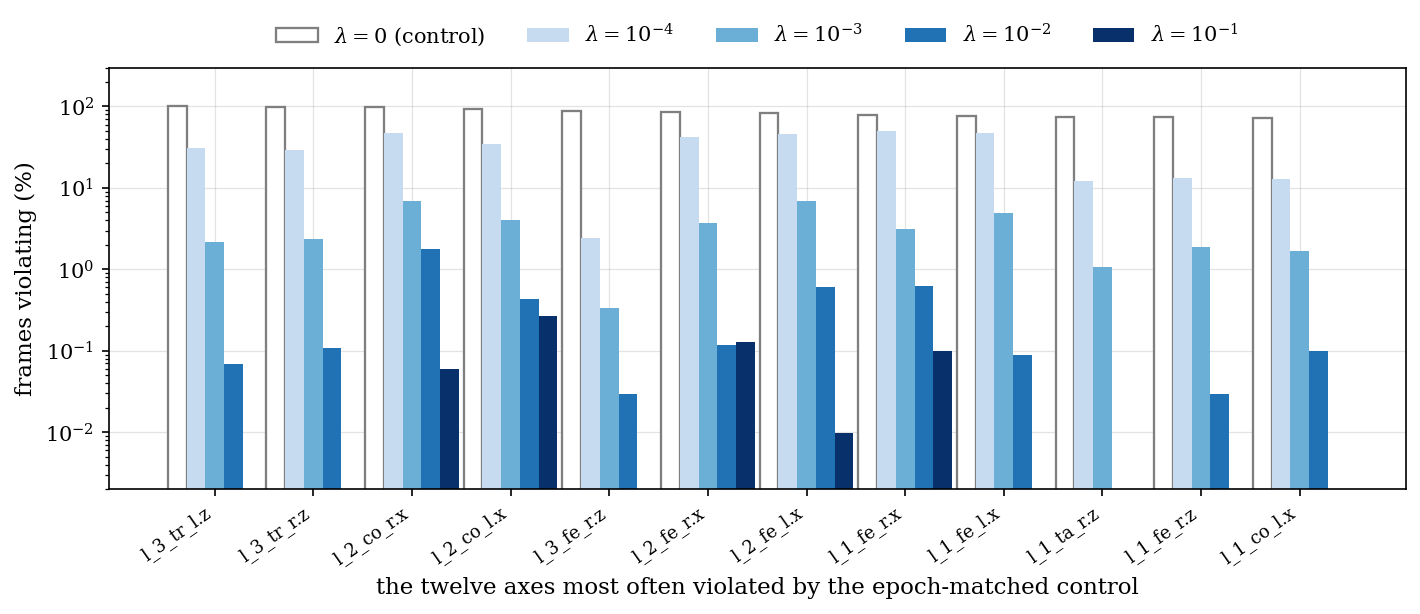
\includegraphics[width=0.92\textwidth]{fig_mv_worst_axes.pdf}
\caption{The twelve axes most frequently violated by the multi-view reference
arm, and their violation rate under each $\lam$ (log scale; bars below
\SI{0.002}{\percent} are drawn at the axis floor). All twelve are leg axes, as
in the single-view case, but the distribution is more extreme: the reference
violates \texttt{l\_3\_tr\_l.z} on \emph{every} test frame and
\texttt{l\_3\_tr\_r.z} on \SI{99.6}{\percent} of them. At $\lam = 10^{-1}$ both
axes are clean on every frame.}
\label{fig:worst}
\end{figure}

\Cref{fig:worst} shows where the violations are concentrated. All twelve of the
most-violated axes belong to the legs, and the trochanter, coxa and femur axes
dominate --- the degrees of freedom that carry stance and swing. The two
third-leg trochanter $z$ axes are violated on essentially every frame, which is
the signature of a systematic offset between the authored range and the pose
the network converges to for that joint, not of occasional bad frames. This is
worth separating from the rest: an axis violated on \SI{100}{\percent} of
frames is evidence about either the model's parameterisation or the authored
limit itself, and the prior resolves it by moving the model, not by
interrogating the limit.

\subsection{Accuracy}
\label{sec:res-acc}

This is where the multi-view result departs from the single-view one. Read
column-wise in \Cref{tab:main}, there is no ambiguity to resolve: the
unregularised reference is the best arm on MPJPE, median MPJPE, PCK at both
resolutions and mean 2D error, and accuracy degrades monotonically with $\lam$
from the reference onward:

\begin{center}
\begin{tabular}{lccccc}
\toprule
 & $\lam=0$ & $10^{-4}$ & $10^{-3}$ & $10^{-2}$ & $10^{-1}$ \\
\midrule
MPJPE (mm)            & 0.9639 & 0.9920 & 1.0750 & 1.1414 & 1.2111 \\
\quad vs.\ reference  & ---    & $+\SI{2.9}{\percent}$ & $+\SI{11.5}{\percent}$ & $+\SI{18.4}{\percent}$ & $+\SI{25.6}{\percent}$ \\
PCK@5\,px (native)    & 0.3350 & 0.3260 & 0.2862 & 0.2511 & 0.2355 \\
\quad vs.\ reference  & ---    & $-\SI{2.7}{\percent}$ & $-\SI{14.6}{\percent}$ & $-\SI{25.0}{\percent}$ & $-\SI{29.7}{\percent}$ \\
Mean 2D error (px)    & 8.725  & 8.985  & 9.724  & 10.319 & 10.942 \\
\bottomrule
\end{tabular}
\end{center}

A least-squares fit of MPJPE against $\log_{10}\lam$ over the four
epoch-matched points gives a slope of \SI{0.0724}{\milli\metre} per decade
($R^2 = 0.998$), against \SI{0.0244}{\milli\metre} per decade ($R^2 = 0.98$)
in single-view --- a factor of $3.0$ in absolute terms and, normalised by each
arm's own reference, $\SI{7.5}{\percent}$ per decade against
$\SI{2.2}{\percent}$. The multi-view model pays roughly three times as much per
decade of regularisation, and it pays from the first decade rather than from a
lower baseline.

\begin{figure}[t]
\centering
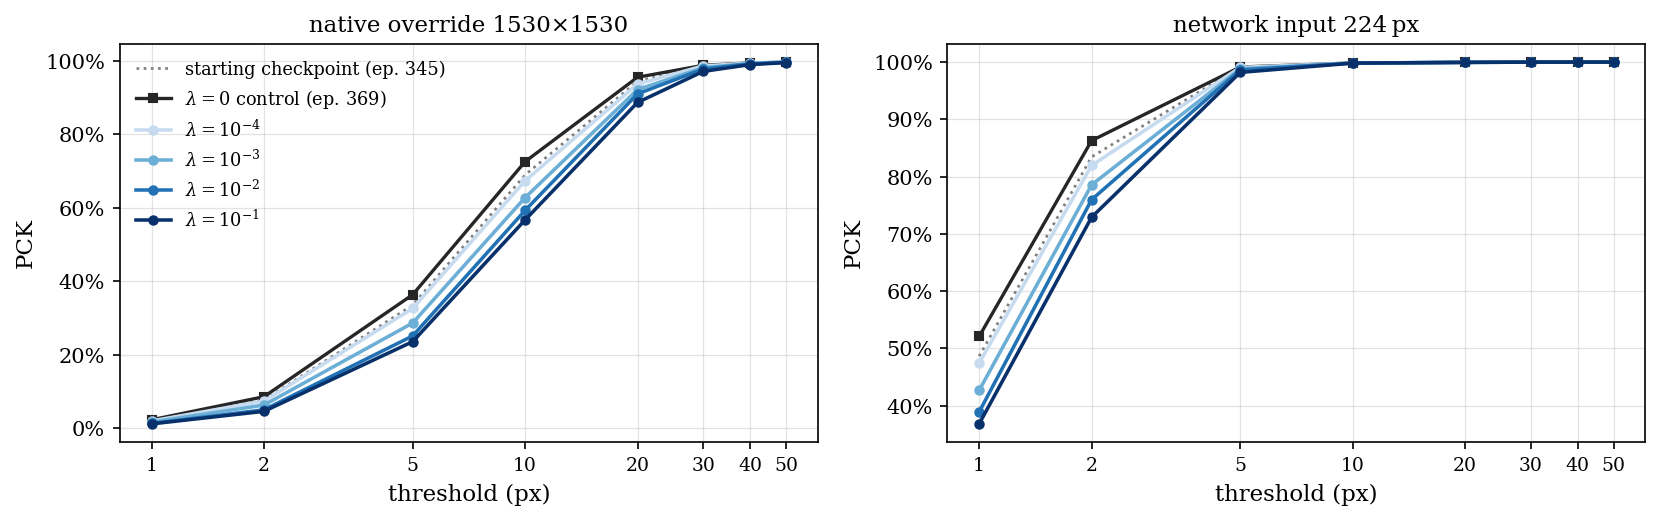
\includegraphics[width=\textwidth]{fig_mv_pck.pdf}
\caption{PCK curves on the multi-view test split at both reporting resolutions.
The five arms are ordered by $\lam$ at every threshold on both curves, with the
unregularised reference uppermost throughout. The ordering is strict: no
constrained arm crosses the reference anywhere, at any threshold, on either
curve.}
\label{fig:pck}
\end{figure}

\Cref{fig:pck} confirms that this is not an artefact of a single threshold.
On both PCK curves the five arms are ordered by $\lam$ at every point, and the
reference dominates all four constrained arms everywhere. Compare the
single-view case, where the reference was beaten at almost every threshold by
the three weakest constrained arms: the qualitative picture is inverted, and it
is inverted despite the constrained arms here having received $24$ epochs of
training that the reference did not.

\begin{figure}[t]
\centering
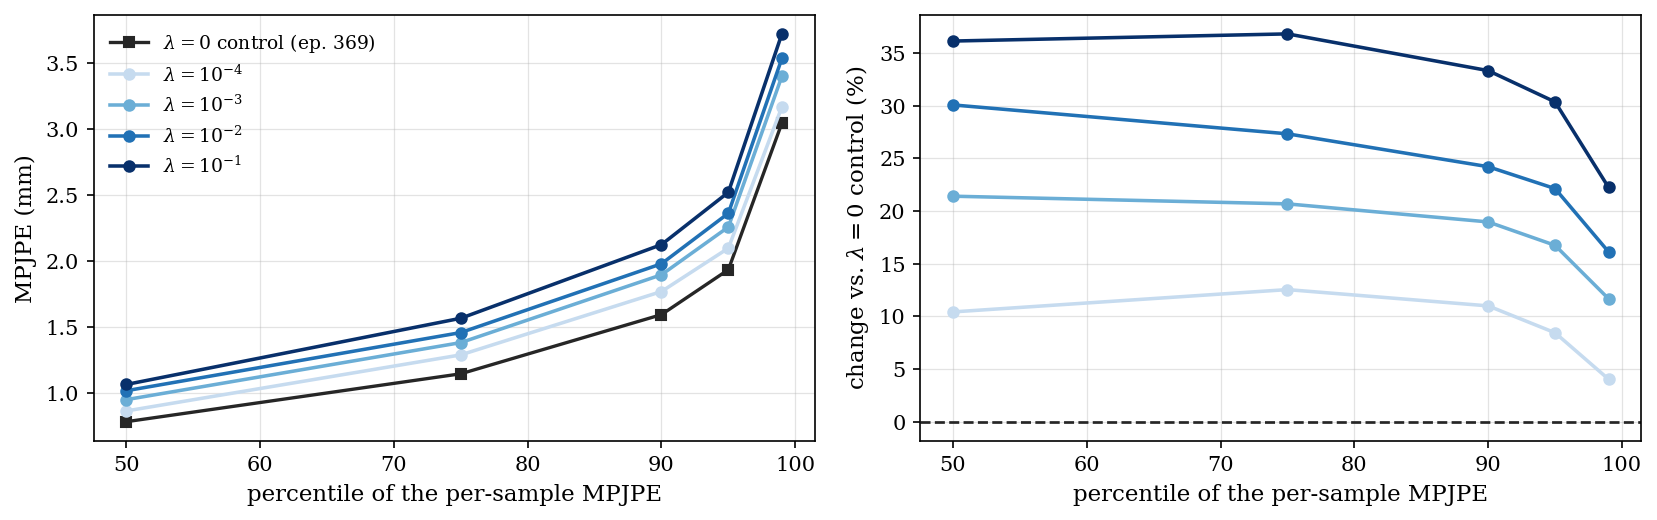
\includegraphics[width=\textwidth]{fig_mv_mpjpe_quantiles.pdf}
\caption{Left: MPJPE quantile functions. Right: change relative to the
reference arm at each percentile. The penalty raises the error by a roughly
constant \emph{relative} amount across the whole distribution --- for
$\lam = 10^{-1}$, $+\SI{26.7}{\percent}$ at P50 against
$+\SI{22.0}{\percent}$ at P99 --- rather than concentrating in the tail where
the implausible poses live.}
\label{fig:quant}
\end{figure}

\Cref{fig:quant} decomposes the 3D error by percentile, and the shape of the
degradation is diagnostic. If the prior were mainly suppressing rare,
grossly implausible predictions, the cost --- and any benefit --- should
concentrate in the upper tail. Instead the relative penalty is largest at the
median ($+\SI{26.7}{\percent}$ at P50 for $\lam = 10^{-1}$) and smallest at P99
($+\SI{22.0}{\percent}$), i.e.\ the prior applies a near-uniform tax on the
typical prediction. That is the profile of a term competing with the data on
ordinary frames, not of a term correcting outliers.

\subsection{Range of motion}
\label{sec:res-rom}

\begin{table}[t]
\centering
\small
\caption{Mean range of motion per bounded axis (deg), by joint group, over the
$129$ axes with a finite authored range. The clipping bound (\Cref{eq:clip}) is
the ROM the reference arm would retain if its trajectory were merely clipped
into the authored box. The single-view reference figure from \cite{sv} is given
in the last column for scale.}
\label{tab:rom}
\begin{tabular}{l r *{5}{r} r}
\toprule
Joint group & axes & $\lam{=}0$ & $10^{-4}$ & $10^{-3}$ & $10^{-2}$ & $10^{-1}$ & \svref{} \\
\midrule
Coxa            & 18 & 70.0 & 69.1 & 61.9 & 55.7 & 51.6 & 78.1 \\
Trochanter      & 18 & 39.0 & 34.7 & 30.9 & 28.7 & 26.3 & 74.2 \\
Femur           & 18 & 59.8 & 44.0 & 24.9 & 18.6 & 16.5 & 71.6 \\
Tibia           & 18 & 39.5 & 33.2 & 29.0 & 24.7 & 21.4 & 88.9 \\
Tarsus          & 18 & 61.1 & 48.4 & 41.3 & 37.2 & 32.7 & 96.3 \\
Antenna         & 18 & 36.2 & 32.7 & 31.4 & 30.5 & 29.5 & 40.9 \\
Head / wings    & 21 & 21.0 & 17.4 & 15.1 & 13.2 & 12.4 & 20.2 \\
\midrule
\textbf{All}    & \textbf{129} & \textbf{46.1} & \textbf{39.4} & \textbf{33.1} & \textbf{29.4} & \textbf{26.9} & \textbf{66.1} \\
\midrule
\multicolumn{2}{l}{\emph{Clipping bound}} & \multicolumn{5}{c}{$30.5$ (mean over all $129$ axes)} & $37.0$ \\
\multicolumn{2}{l}{\emph{Mean authored range}} & \multicolumn{5}{c}{$51.6$} & $51.6$ \\
\bottomrule
\end{tabular}
\end{table}

The multi-view reference is already markedly more conservative than the
single-view one. It moves through a mean ROM of \SI{46.1}{\degree} per bounded
axis against \SI{66.1}{\degree} in single-view, for the same mean authored
range of \SI{51.6}{\degree}: a ratio of means of $0.89\times$ against
$1.28\times$. Per axis the picture is the same --- mean ratio $1.34$ against
$1.95$, median $0.91$ against $1.18$, and $56$ of $129$ axes exceeding their
authored range against $79$ (\Cref{fig:ratio}). Multi-view geometry, without
any anatomical supervision, already places the typical joint inside its
authored envelope; what remains is a smaller number of axes that are outside it
badly and persistently.

Clipping the multi-view reference trajectory into the box would leave
\SI{30.5}{\degree}. The trained arms give $39.4$, $33.1$, $29.4$ and
\SI{26.9}{\degree} for $\lam = 10^{-4} \ldots 10^{-1}$ (\Cref{tab:rom}). From
$\lam = 10^{-2}$ upward, therefore, the model again withdraws into the interior
of the feasible set, ending at $\lam = 10^{-1}$ some \SI{12}{\percent} below
the clipping bound. Since \Cref{eq:penalty} has zero gradient there, this is
not a direct response to the penalty, and the learned-margin explanation of
\cite{sv} carries over unchanged: predicting conservatively is the cheapest way
to keep the expected hinge loss at zero when one's own predictions carry noise.

\begin{figure}[t]
\centering
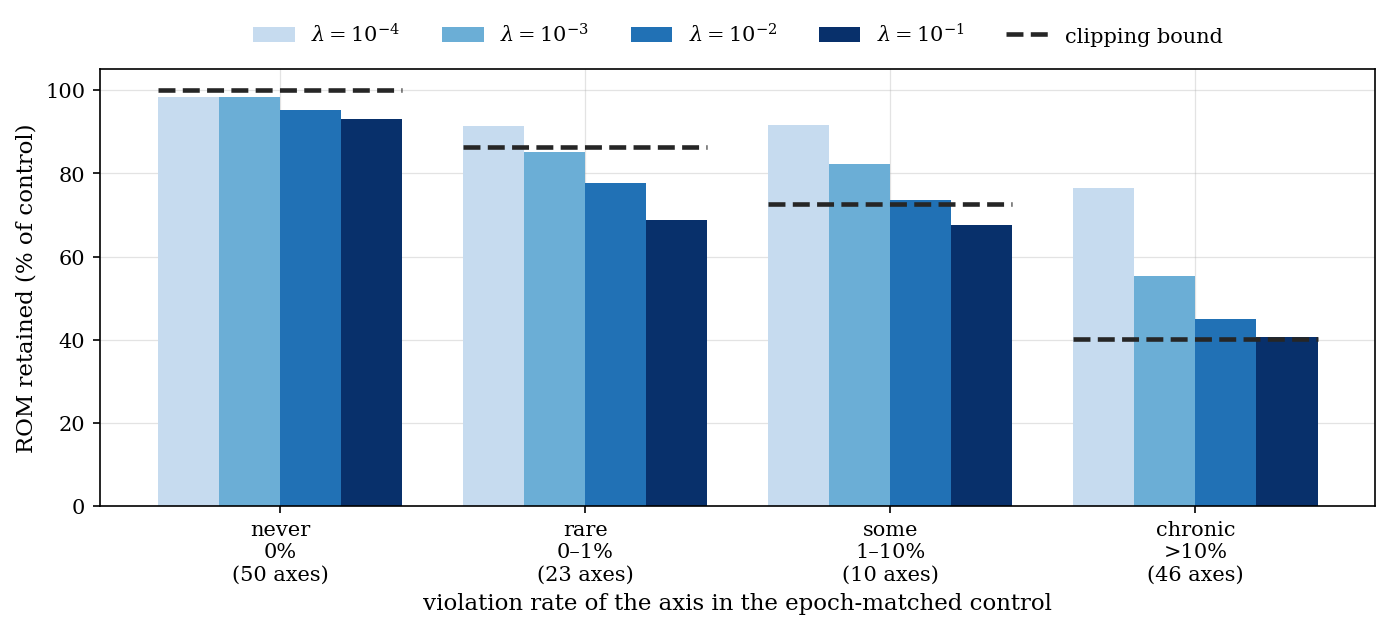
\includegraphics[width=0.86\textwidth]{fig_mv_rom_retention.pdf}
\caption{ROM retained relative to the multi-view reference, with axes grouped
by the reference's own violation rate on that axis. The dashed rule in each
group is the clipping bound of \Cref{eq:clip}. Axes that never violated retain
\SIrange{92.4}{98.4}{\percent} of their range at every $\lam$. On chronically
violating axes, $\lam = 10^{-1}$ lands on the clipping bound
(\SI{40.3}{\percent} vs.\ \SI{40.4}{\percent}) --- one decade higher than in
single-view, where $\lam = 10^{-2}$ already reached it.}
\label{fig:retention}
\end{figure}

\Cref{fig:retention} resolves the effect by axis severity. Three readings
follow. First, the prior is \emph{well targeted}: the $53$ axes that never
violated in the reference retain \SIrange{92.4}{98.4}{\percent} of their range
at every $\lam$, so the penalty is not indiscriminately damping the whole pose;
targeting is in fact slightly better than in single-view, where the same bucket
retained \SIrange{93.6}{95.8}{\percent} from a much smaller set of $33$ axes.
Second, it \emph{overshoots on marginal axes}, exactly as before: on axes that
violated on less than \SI{1}{\percent} of frames, $\lam = 10^{-1}$ retains
\SI{69.3}{\percent} of the reference range where clipping would retain
\SI{85.8}{\percent} --- $17$ percentage points of motion removed for which no
violation can account. Third, the alignment between the sweep and the clipping
bound is shifted by one decade: chronic axes reach the bound at
$\lam = 10^{-1}$ here and at $\lam = 10^{-2}$ in single-view, which is a direct
consequence of the multi-view data term resisting the same penalty more
strongly.

\begin{figure}[t]
\centering
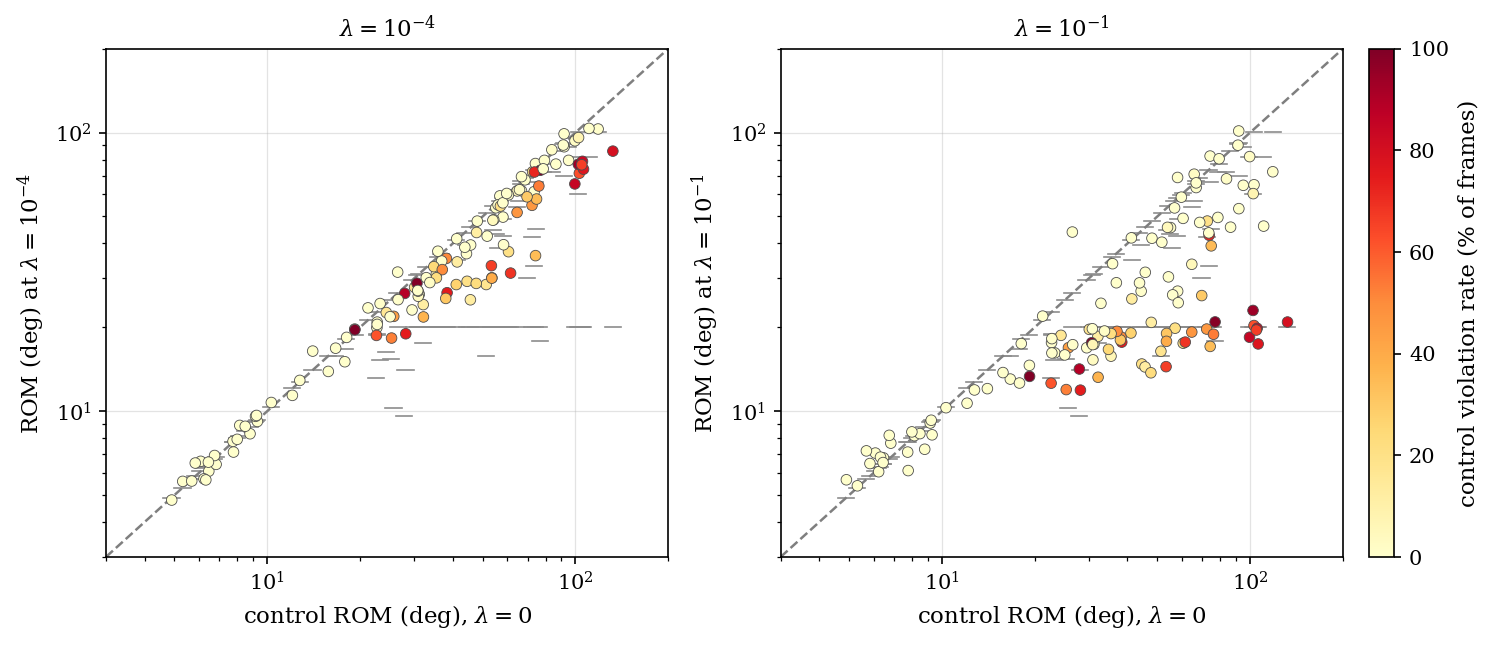
\includegraphics[width=\textwidth]{fig_mv_rom_scatter.pdf}
\caption{Per-axis ROM before and after regularisation (log--log). Marker colour
encodes the reference violation rate; horizontal ticks mark the clipping bound
for each axis. At $\lam = 10^{-4}$ most axes sit near or above their clipping
bound and the low-ROM axes are essentially untouched. At $\lam = 10^{-1}$ a
dense band has collapsed to roughly \SIrange{12}{20}{\degree} regardless of its
starting ROM or of whether it ever violated --- the same visual signature of a
learned margin reported in the single-view study, at a slightly lower plateau.}
\label{fig:scatter}
\end{figure}

\begin{figure}[t]
\centering
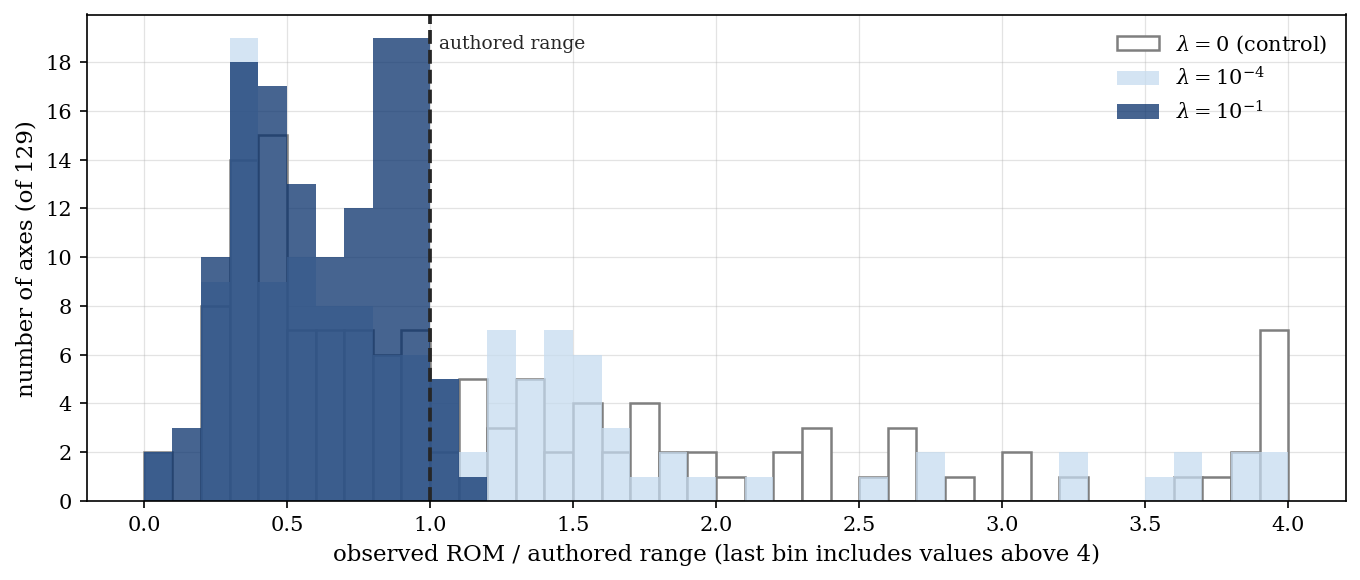
\includegraphics[width=0.86\textwidth]{fig_mv_rom_ratio.pdf}
\caption{Distribution over the $129$ bounded axes of the ratio between observed
ROM and authored range. The multi-view reference (mean $1.34$, median $0.91$;
$56$ axes above $1.0$) already sits close to the authored envelope, unlike the
single-view reference (mean $1.95$, median $1.18$; $79$ axes). By
$\lam = 10^{-1}$ only $6$ axes reach the envelope and the mean ratio is $0.62$:
the typical joint uses well under two-thirds of the range it is permitted.}
\label{fig:ratio}
\end{figure}

\Cref{fig:scatter,fig:ratio} display the same phenomenon per axis and in
distribution, and \Cref{tab:rom} shows where it is paid for. Femur ROM falls
from \SI{59.8}{\degree} to \SI{16.5}{\degree} ($-\SI{72}{\percent}$), tarsus by
\SI{46}{\percent} and tibia by \SI{46}{\percent}, while coxa loses only
\SI{26}{\percent} and antennae \SI{19}{\percent}. The femur--tibia complex is
the principal locomotor degree of freedom of the stick insect; as in the
single-view case, a model whose femora sweep through less than
\SI{17}{\degree} will render a visibly stiff gait irrespective of its MPJPE.
The concern is sharper here, because the multi-view reference had a defensible
femoral range to begin with and the regularisation removes most of it.

\subsection{Spread versus centre}
\label{sec:res-centre}

The mean absolute shift of the per-axis mean angle relative to the reference is
$3.61$, $4.38$, $4.61$ and \SI{4.75}{\degree} for
$\lam = 10^{-4} \ldots 10^{-1}$. As in single-view, most of this shift is
already present at the weakest setting and grows only slowly thereafter
($+\SI{32}{\percent}$ across three further decades, against
$+\SI{12}{\percent}$ in single-view), so the \emph{centre} of the pose
distribution is largely set by the $24$ epochs of continued training while the
penalty acts on the \emph{spread}. The residual growth with $\lam$ is somewhat
larger than in single-view, consistent with the stronger inward pull documented
in \Cref{sec:res-rom}.

%==============================================================================
\section{Single-view versus multi-view}
\label{sec:compare}

\begin{figure}[t]
\centering
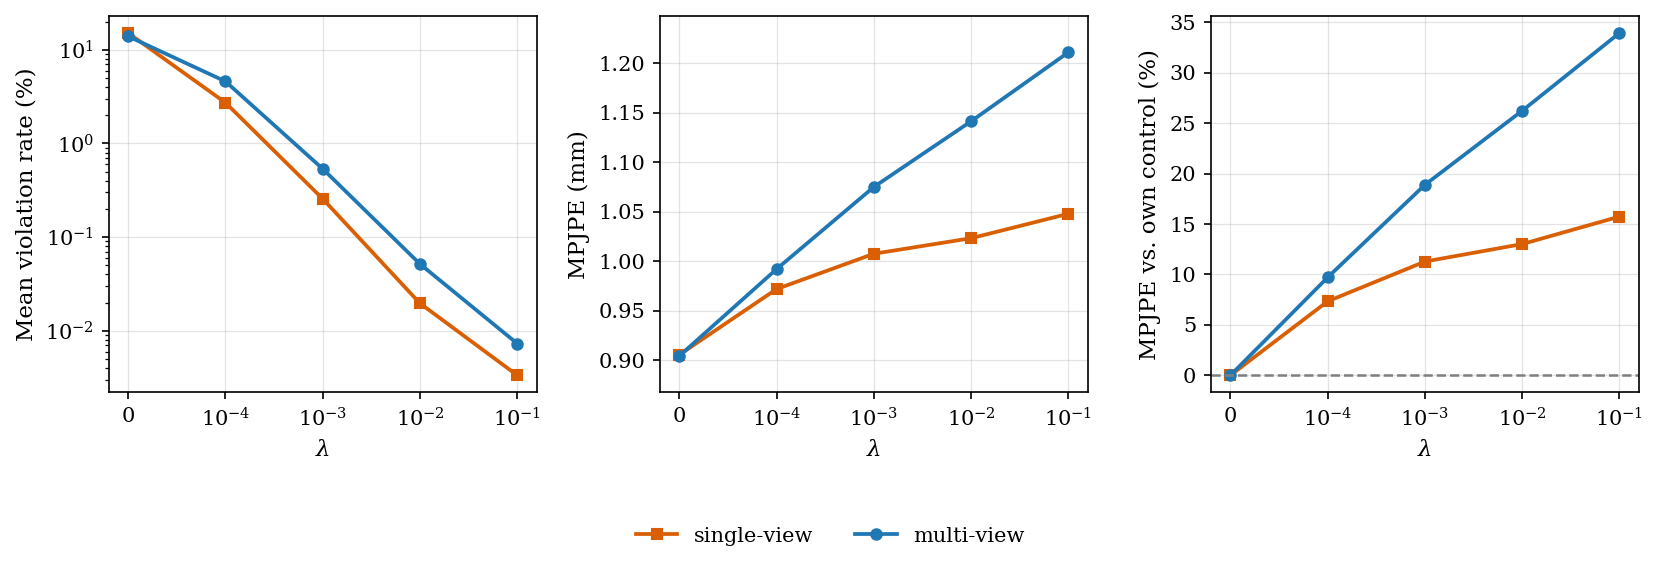
\includegraphics[width=\textwidth]{fig_mv_sv_compare.pdf}
\caption{The two sweeps side by side. Left: mean violation rate; the two modes
start from a nearly identical rate and the multi-view arm reduces it slightly
more slowly at every $\lam$. Centre: absolute MPJPE; the multi-view reference
is the more accurate model but the single-view reference is the least accurate
point of either sweep. Right: MPJPE relative to each mode's own reference,
which is the controlled view --- the single-view curve stays below zero
throughout while the multi-view curve rises immediately.}
\label{fig:compare}
\end{figure}

\Cref{fig:compare} places the two sweeps side by side, and
\Cref{tab:global} collects the comparison in numbers. Four points stand out.

\paragraph{The multi-view reference is the better model, but not by the
expected margin on plausibility.}
It is \SI{11.7}{\percent} better on MPJPE ($0.9639$ vs.\
\SI{1.0920}{\milli\metre}), violates on fewer axes ($76$ vs.\ $96$), and has a
lower worst-case overshoot (\SI{56.6}{\degree} vs.\ \SI{77.7}{\degree}). Yet
its \emph{mean} violation rate is barely lower (\SI{13.96}{\percent} vs.\
\SI{14.76}{\percent}). Multi-view geometry concentrates the implausibility onto
fewer axes and makes it less extreme, but it does not make it rarer. The
hypothesis of \cite{sv} --- that multi-view should have less to fix --- is
therefore only half confirmed: less to fix in \emph{severity} and in
\emph{breadth}, not in \emph{frequency}.

\paragraph{On range of motion, multi-view is much closer to anatomy from the
start.}
Mean ROM per bounded axis is \SI{46.1}{\degree} against \SI{66.1}{\degree}, the
per-axis ROM/authored ratio is $1.34$ against $1.95$, and the median axis is
inside its authored range ($0.91$) rather than outside it ($1.18$). Under the
under-articulation measure recommended in \cite{sv}, the multi-view reference
would be scored as the more anatomically credible model by a wide margin ---
which the violation rate alone does not reveal.

\paragraph{The accuracy cost of the prior is measured, not estimated, and it is
large.}
In the single-view study every constrained arm beat the reference and the
prior's cost had to be inferred from the slope within the epoch-matched arms;
the correct $\lam=0$ control was missing. Here the same design flaw is present
--- the reference again received no additional epochs --- but its direction is
now favourable: continued training can only help the constrained arms, and they
lose anyway, on every metric, at every $\lam$. The measured deltas of
\Cref{tab:global} are therefore \emph{lower bounds} on the cost of the prior in
multi-view. This is the one respect in which the multi-view study is
methodologically stronger than its single-view predecessor.

\paragraph{The cost per decade scales inversely with the strength of the
evidence.}
\SI{0.0724}{\milli\metre} per decade against \SI{0.0244}{\milli\metre}; in
relative terms \SI{7.5}{\percent} against \SI{2.2}{\percent} of each arm's own
reference. Five calibrated views leave a much smaller set of poses consistent
with the image evidence than one view does; a prior that pushes the prediction
out of that set is paid for in full, whereas in the single-view case it can
select within a large equivalence class almost for free.

\begin{table}[t]
\centering
\small
\setlength{\tabcolsep}{3pt}
\caption{Global comparison of the two sweeps. Absolute values for the reference
arms; for the constrained arms, change relative to that mode's own reference
(so that the fine-tuning confound is held fixed within each column pair).
Positive is worse for MPJPE, 2D error, violation rate and overshoot; positive
is better for PCK. Single-view figures are from \cite{sv}; all rows are scored
on the same test split against the same authored ranges.}
\label{tab:global}
\begin{tabular}{l rr rr rr rr}
\toprule
 & \multicolumn{2}{c}{Reference ($\lam = 0$)}
 & \multicolumn{2}{c}{$\lam = 10^{-4}$}
 & \multicolumn{2}{c}{$\lam = 10^{-3}$}
 & \multicolumn{2}{c}{$\lam = 10^{-1}$} \\
\cmidrule(lr){2-3}\cmidrule(lr){4-5}\cmidrule(lr){6-7}\cmidrule(lr){8-9}
Quantity & SV & MV & SV & MV & SV & MV & SV & MV \\
\midrule
\multicolumn{9}{l}{\emph{Anatomical plausibility}}\\
Violating axes (of 162)      & 96 & 76 & $-7$ & $-1$ & $-11$ & $-3$ & $-55$ & $-55$ \\
Mean violation rate (\%)     & 14.76 & 13.96 & $\div 5.4$ & $\div 3.0$ & $\div 57$ & $\div 26$ & $\div 4400$ & $\div 1900$ \\
Max overshoot (deg)          & 77.70 & 56.57 & 50.84 & 43.44 & 25.64 & 17.65 & 2.53 & 3.96 \\
\midrule
\multicolumn{9}{l}{\emph{Accuracy, relative to own reference}}\\
MPJPE (mm)                   & 1.0920 & 0.9639 & $-11.0\%$ & $+2.9\%$ & $-7.7\%$ & $+11.5\%$ & $-4.0\%$ & $+25.6\%$ \\
PCK@5\,px (native)           & 0.3762 & 0.3350 & $+14.3\%$ & $-2.7\%$ & $+7.0\%$ & $-14.6\%$ & $-0.5\%$ & $-29.7\%$ \\
Mean 2D error (px)           & 7.827 & 8.725 & $-7.6\%$ & $+3.0\%$ & $-2.7\%$ & $+11.5\%$ & $+2.7\%$ & $+25.4\%$ \\
\midrule
\multicolumn{9}{l}{\emph{Range of motion, $129$ bounded axes}}\\
Mean ROM (deg)               & 66.1 & 46.1 & 44.0 & 39.4 & 37.3 & 33.1 & 30.3 & 26.9 \\
ROM retained (\% of ref.)    & --- & --- & 71.0 & 88.8 & 63.4 & 79.4 & 56.1 & 68.1 \\
Mean ROM / authored range    & 1.95 & 1.34 & --- & 1.08 & --- & 0.81 & 0.66 & 0.62 \\
Axes above authored range    & 79 & 56 & --- & 52 & --- & 43 & 15 & 6 \\
\midrule
\multicolumn{9}{l}{\emph{Derived}}\\
Clipping bound (deg)         & \multicolumn{2}{c}{$37.0$ \quad / \quad $30.5$} & \multicolumn{6}{c}{} \\
MPJPE slope (mm/decade)      & \multicolumn{2}{c}{$0.0244$ \quad / \quad $0.0724$} & \multicolumn{6}{c}{$R^2 = 0.98$ \quad / \quad $R^2 = 0.998$} \\
$\lam$ reaching clip.\ bound & \multicolumn{2}{c}{$10^{-2}$ \quad / \quad $10^{-1}$} & \multicolumn{6}{c}{on chronically violating axes} \\
\bottomrule
\end{tabular}
\end{table}

%==============================================================================
\section{Discussion}
\label{sec:discussion}

\subsection{The fine-tuning confound, and why it points the other way here}
\label{sec:disc-confound}

Every ``constrained versus reference'' comparison in both studies contrasts
\emph{prior plus continued training} against \emph{neither}: the correct
control, $\lam = 0$ continued for the same epochs, was excluded from the design
of the sweep. In the single-view study this was fatal to the headline claim,
because the constrained arms won and the win could be attributed to either
factor.

In the multi-view study the same omission has the opposite consequence. The
constrained arms received $24$ epochs the reference did not, and they still
lose on every accuracy metric at every $\lam$. Continued training on this
dataset improves accuracy --- that is the lesson of the single-view sweep, where
$49$ extra epochs bought roughly \SI{0.12}{\milli\metre} of MPJPE at
$\lam = 10^{-4}$ --- so the honest, control-matched cost of the prior in
multi-view is \emph{at least} the $+\SI{2.9}{\percent}$ to
$+\SI{25.6}{\percent}$ of \Cref{tab:main}, and plausibly more. The missing
control would sharpen the estimate; it cannot overturn the sign.

A single multi-view run at $\lam = 0$ continued to epoch $369$ would still be
worth having, both to quantify the gap and to make the two studies symmetric.
It is the cheapest remaining experiment in the design.

\subsection{Why the multi-view model resists the prior}
\label{sec:disc-mechanism}

Three observations point at the same mechanism. The multi-view reference is
already inside the authored envelope on the typical axis
(\Cref{fig:ratio}); the penalty's cost per decade is three times larger
(\Cref{sec:res-acc}); and the cost is spread uniformly over the error
distribution rather than concentrated in the tail (\Cref{fig:quant}).

The reading these support is that a prior of this kind pays for itself only
where the data underdetermines the answer. With one view, many joint
configurations reproject to nearly identical evidence, and the network is free
to pick among them by criteria unrelated to anatomy; a prior that restricts
that choice removes implausible poses without contradicting the image. With
five calibrated views, triangulation has already narrowed the set of consistent
poses to something close to a point, and the residual disagreement between the
authored box and the prediction is no longer free choice --- it is a genuine
conflict between the authored limits and the evidence. Regularising it away
moves the prediction off the data, which is exactly what \Cref{fig:quant}
measures.

This reading has an uncomfortable corollary, and it should be stated plainly:
where the multi-view model persistently violates a limit --- \texttt{l\_3\_tr\_l.z}
on \SI{100}{\percent} of frames, \texttt{l\_2\_co\_r.x} on \SI{98}{\percent}
--- the conflict may be evidence \emph{against the authored range}, or against
the joint's rotation parameterisation, rather than against the model. Five
cameras agreeing on a configuration outside the authored box is a different
kind of signal from one camera guessing one. The authored limits were set by
hand and have not been validated against the multi-view reconstruction; the
axes of \Cref{fig:worst} are the natural place to start.

\subsection{Over-regularisation and the learned margin}

The failure mode identified in \cite{sv} reproduces here in full. A one-sided
hinge is by construction inactive inside the feasible set, yet for
$\lam \ge 10^{-2}$ the multi-view model settles well inside it
(\Cref{sec:res-rom}), and \Cref{fig:scatter} shows a dense band of axes
collapsing to a common \SIrange{12}{20}{\degree} plateau irrespective of their
starting ROM. The two candidate mechanisms are unchanged: (a) prediction noise
makes a near-boundary configuration risky in expectation, so the minimum-risk
prediction sits at a margin; (b) the penalty is a batch mean, so a systematic
inward bias across many axes is a cheap way to reduce it.

The multi-view data offer one new discriminating observation. The plateau is at
a \emph{lower} absolute ROM than in single-view (\SIrange{12}{20}{\degree}
against \SIrange{15}{25}{\degree}) even though the multi-view model is the more
accurate --- and therefore, presumably, the less noisy --- of the two. That is
mildly against mechanism (a) taken alone, and suggests that the batch-mean
argument (b) contributes materially: the multi-view head predicts one pose per
sample rather than one per view, so a given inward bias is a cheaper way to
lower the batch mean there than in single-view.

\subsection{Limitations of the plausibility metric}

The violation rate is minimised by a stiff pose, and \Cref{sec:res-rom} shows
the sweep exploiting exactly that degree of freedom, so a plausibility claim
resting on the violation rate alone is not sound in either mode. Pairing it
with the per-axis ratio of observed ROM to authored range (\Cref{fig:ratio})
is what makes the comparison of \Cref{sec:compare} informative: under that
measure the multi-view reference, with a median ratio of $0.91$, is already the
more plausible model, and the $\lam = 10^{-1}$ arm, with a mean ratio of
$0.62$, has over-corrected.

\subsection{Choice of operating point}

The multi-view trade-off is much harsher than the single-view one, and no
setting is free. The recommendation depends on what the model is for:

\begin{description}[leftmargin=1.4em,style=nextline,itemsep=0.35em]
\item[Accuracy-critical use --- $\lam = 10^{-4}$, or none at all.]
  $+\SI{2.9}{\percent}$ MPJPE and $-\SI{2.7}{\percent}$ PCK@5\,px is the only
  cost in this sweep that could be described as small, but it still leaves a
  \SI{43.4}{\degree} maximum overshoot and \SI{4.6}{\percent} of frames
  violating. If plausibility is not an explicit requirement, the unregularised
  reference remains the best multi-view model on every accuracy metric
  measured.
\item[Balanced use --- $\lam = 10^{-3}$ (recommended default).]
  Violation rate \SI{0.54}{\percent}, maximum overshoot \SI{17.6}{\degree}, ROM
  above the clipping bound (\SI{33.1}{\degree} vs.\ \SI{30.5}{\degree}), at
  $+\SI{11.5}{\percent}$ MPJPE. This is the strongest setting that has not yet
  begun withdrawing into the interior of the feasible set.
\item[Hard plausibility requirement --- $\lam = 10^{-2}$.]
  The weakest setting at which no anatomically impossible pose survives
  (maximum overshoot \SI{4.9}{\degree}), at $+\SI{18.4}{\percent}$ MPJPE and
  $-\SI{25.0}{\percent}$ PCK@5\,px. Note that this is where the single-view
  study placed its default; in multi-view the same choice costs roughly three
  times as much.
\item[Not recommended --- $\lam = 10^{-1}$.]
  Its marginal plausibility gain over $10^{-2}$ is negligible
  (\SI{4.9}{\degree} to \SI{4.0}{\degree} of maximum overshoot) while it costs
  a further \SI{7}{\percent} of MPJPE and \SI{72}{\percent} of femur range.
\end{description}

\subsection{Threats to validity}

Three caveats bound the conclusions. First, the missing $\lam = 0$ control
(\Cref{sec:disc-confound}); its direction is favourable here but its magnitude
is unmeasured. Second, the multi-view fine-tune is $24$ epochs against the
single-view study's $49$, so the two sweeps are not matched on continuation
budget --- this affects the size of the confound in each, not the sign of the
within-sweep trends, but it should be kept in mind when reading
\Cref{tab:global} row by row. Third, ROM as defined here is a min--max
statistic over the test set and is therefore sensitive to outliers; the
distributional view of \Cref{fig:ratio} and the per-axis view of
\Cref{fig:scatter} are provided so that the aggregate is not read in isolation.

%==============================================================================
\section{Conclusion}
\label{sec:conclusion}

Returning to the question of \Cref{sec:intro}:

\begin{description}[leftmargin=1.4em,style=nextline]
\item[The prior still works on what it penalises --- yes.]
  Across four decades it reduces the mean violation rate by between $3.0\times$
  and $1900\times$ and the worst overshoot from \SI{56.6}{\degree} to
  \SI{4.0}{\degree}, acting on precisely the trochanter, coxa and femur axes
  that dominate locomotion.
\item[Is it worthwhile in multi-view --- on this evidence, no.]
  The unregularised reference is the most accurate arm on MPJPE, median MPJPE,
  PCK at both resolutions and mean 2D error, and it holds that position at
  every $\lam$ despite the constrained arms having received $24$ additional
  epochs of training. The cost is \SI{7.5}{\percent} of MPJPE per decade of
  $\lam$, three times the single-view figure.
\item[Was the hypothesis of \cite{sv} confirmed --- partially.]
  Multi-view does have less to fix, but in severity and breadth rather than in
  frequency: fewer violating axes ($76$ vs.\ $96$), a lower worst overshoot
  (\SI{56.6}{\degree} vs.\ \SI{77.7}{\degree}) and a far more anatomical range
  of motion (ROM/authored ratio $1.34$ vs.\ $1.95$), but a nearly identical
  mean violation rate.
\end{description}

The two studies together support a single statement that neither supports
alone: \emph{the value of an authored anatomical prior is inversely related to
the strength of the geometric evidence available to the model}. Where evidence
is weak the prior selects among poses the data cannot distinguish, and is
nearly free; where evidence is strong the prior contradicts the data, and is
paid for in full. The corollary for the SMILify pipeline is that the prior
belongs in the single-view branch, and that in the multi-view branch the
persistent violations are better read as a question about the authored limits
than as a defect of the model.

%==============================================================================
\section{Next step}
\label{sec:next}

\begin{enumerate}[leftmargin=1.9em,itemsep=0.45em]

\item Run the missing control: multi-view $\lam = 0$ continued to epoch $369$,
      to convert the lower bounds of \Cref{tab:global} into measured deltas.
\item Audit the authored ranges on the axes of \Cref{fig:worst}, starting with
      \texttt{l\_3\_tr\_\{l,r\}.z} and \texttt{l\_2\_co\_r.x}, against the
      multi-view reconstruction. An axis violated on \SI{100}{\percent} of
      frames by a five-camera model is a hypothesis about the limit, not only
      about the model.
\item Test a tolerance band --- penalise only beyond $[\,m_a + \epsilon,\,
      M_a - \epsilon\,]$ with $\epsilon < 0$, i.e.\ a soft margin outside the
      box --- and an annealed $\lam$, to separate the learned-margin effect
      from violation removal and to recover the range of motion lost inside the
      feasible set.
\item Add the under-articulation measure (ROM/authored ratio) to the sweep
      tables as a first-class plausibility metric, so that a stiff model cannot
      score as a plausible one.
\item Extend both sweeps to $5{\times}10^{-2}$, $5{\times}10^{-1}$, $1$, $5$
      and $10$ for completeness, at low priority: both curves are already
      saturated in plausibility and monotone in cost.
\end{enumerate}

%==============================================================================
\appendix
\section{Data provenance}
\label{app:prov}

\begin{description}[leftmargin=0em,style=nextline,itemsep=0.25em,font=\normalfont\ttfamily\small]
\item[prior\_study\_results/sweep/\{sweep.csv, arms.csv, comparison.md\}]
  Aggregated sweep metrics for both modes; source of the violation and MPJPE
  columns of \Cref{tab:main,tab:global}.
\item[prior\_study\_results/*/mv\_constrained/analysis/]
  Together with the matching \texttt{mv\_reference} directory: per-arm
  \texttt{limit\_violations.csv}, \texttt{per\_axis\_stats.csv},
  \texttt{magnitude\_stats.csv} and \texttt{baseline\_summary.md}; source of
  all ROM, retention and centre-shift analyses.
\item[prior\_study\_results/*/sv\_constrained/analysis/]
  The single-view counterparts, used only for the comparison of
  \Cref{sec:compare}.
\item[benchmark\_multiview\_*/benchmark\_report.txt]
  Per-arm PCK curves, 2D errors and MPJPE percentiles, one directory per arm
  on the \texttt{\dots FIXED} benchmark run; source of
  \Cref{fig:pck,fig:quant}.
\item[3D\_model\_prep/SMILy\_STICK\_limits\_authored.pkl]
  Authored per-joint rotation limits (\texttt{joint\_limits}), against which all
  arms in both studies are scored.
\item[report\_joint\_limit\_prior/make\_mv\_figures.py]
  Script regenerating every figure in this report from the sources above.
\end{description}

\noindent
The clipping bound (\Cref{eq:clip}), the ROM retention buckets
(\Cref{fig:retention}), the joint-group aggregation (\Cref{tab:rom}) and the
cross-mode normalisation of \Cref{tab:global} are derived in this report and in
\cite{sv}, and are not present in the original sweep outputs.

%==============================================================================
\begin{thebibliography}{9}
\bibitem{sv}
Y.~Anouar.
\newblock \emph{Effect of an Authored Joint-Limit Prior on Single-View 3D Pose
Regression of the Stick Insect: A regularisation sweep on the SMILySTICKS
benchmark}.
\newblock Forschungszentrum J\"ulich --- SMILify project, 3 September 2026.
\newblock \texttt{report\_joint\_limit\_prior/sv\_study.tex}.
\end{thebibliography}

\end{document}
